\chapter{Diseño de firmware}
En este capítulo se presentan todas las etapas necesarias para el desarrollo de un sistema de adquisición de datos capaz de generar una imagen. Estas etapas incluyen la caracterización de resistencias y fotorresistencias, así como la implementación final del sistema de adquisición de datos. También, se describe el diseño digital correspondiente a cada una de estas fases. Para obtener la imagen, se diseñó una PCB destinada a una matriz de fototransistores, cuyo diseño también se explicará en detalle.

\section{Caracterización de resistencias}
\subsection{Caracterización de resistencia}
En esta etapa, se realizó la caracterización de resistencias utilizando un circuito divisor de voltaje (Figura \ref{fig:divisor2}). En este circuito, $R_{test}$ simula la resistencia de un pixel de un arreglo de microbolómetros, mientras que $R_{ref}$ emula un circuito de lectura. Se probaron distintos valores de $R_{test}$ con el fin de imitar un microbolómetro bajo la influencia de luz y así analizar que valor de $R_{Ref}$ es el más adecuado para cualquier $R_{test}$. Esta fase inicial se centró en la caracterización de resistencias fijas para obtener una visión general de los módulos necesarios para caracterizar un microbolómetro. Además, trabajar con resistencias de valores conocidos permite verificar con mayor precisión si los resultados experimentales coinciden con los teóricos.

            \begin{figure}[hbtp]
                \centering
                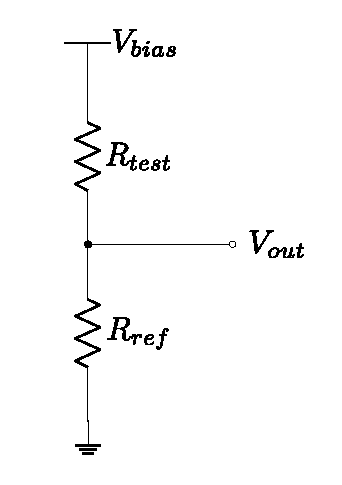
\includegraphics[width=0.3\textwidth]{divisor2}
                \caption{Divisor de voltaje como microbolómetro y circuito de lectura}
                \label{fig:divisor2}
            \end{figure} 
\newpage
Para determinar cuál es el valor más adecuado de $R_{ref}$ para cualquier $R_{test}$, se llevó a cabo una simulación de dos circuitos en LTSpice. En ambos circuitos, se realizó un barrido de $R_{test}$ desde $1k\Omega$ hasta $10k\Omega$, con incrementos de $1k\Omega$. La única diferencia entre los circuitos fue el valor de $R_{ref}$: en uno de ellos, $R_{ref}$ se fijó en $1k\Omega$, mientras que en el otro se estableció en $10k\Omega$. Esta comparación permitió evaluar cómo afectaba el valor de $R_{ref}$ en la respuesta del sistema ante distintos valores de $R_{test}$, facilitando la selección del valor más adecuado para optimizar la lectura del circuito.
            \begin{figure}[hbtp]
                \centering
                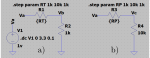
\includegraphics[width=0.9\textwidth]{cto_ltspice}
                \caption{Divisores de voltaje para la elección de $R_{ref}$}
                \label{fig:cto_ltspice}
            \end{figure}

En las Figuras \ref{fig:graph_1k} y \ref{fig:graph_10k} se presentan los resultados de los barridos de Rtest. Supongase que en lugar de tener resistencias conocidas, se emplea un microbolómetro cuya resistencia no se puede medir directamente, salvo a través del circuito de lectura con $R_{ref}$, y despejando la ecuación del divisor de voltaje. Al polarizar el circuito divisor con voltajes muy bajos, resulta imposible identificar con precisión la resistencia del detector. No obstante, al polarizar a partir de $2.7V$, se vuelve más fácil determinar el valor de $R_{test}$.

            \begin{figure}[hbtp]
                \centering
                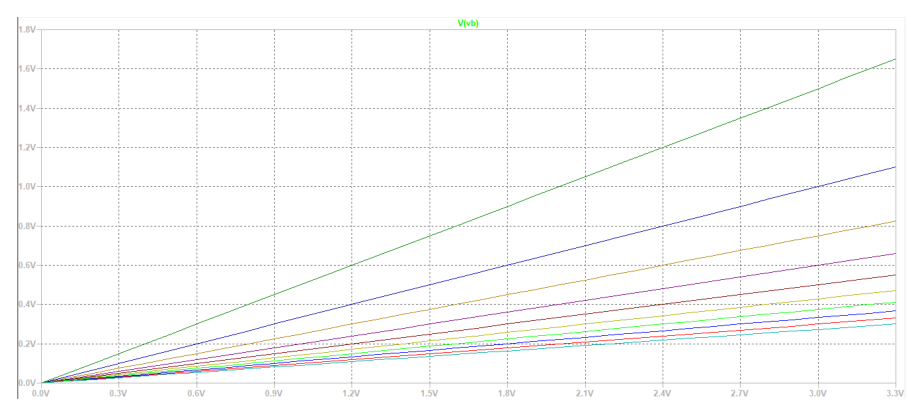
\includegraphics[width=1\textwidth]{graph_1k}
                \caption{Gráficas de voltaje de $R_{ref} = 1k\Omega$ con barrido en $R_{test}$}
                \label{fig:graph_1k}
            \end{figure}
            
 Sin embargo, es importante señalar que la influencia de $R_{ref}$ también juega un papel crucial. En la Figura \ref{fig:graph_1k}, con $R_{ref} = 1k\Omega$, se observa que, para valores altos de $R_{test}$, resulta difícil conocer con precisión la resistencia del detector, siendo únicamente posible identificarla para valores menores a $6k\Omega$. En contraste, en la Figura \ref{fig:graph_10k}, donde $R_{ref} = 10k\Omega$, las curvas no se empalman y es más sencillo identificar la resistencia del detector, lo que llevó a optar por un valor de $R_{ref} = 10k\Omega$ para la caracterización de resistencias.
 
            \begin{figure}[hbtp]
                \centering
                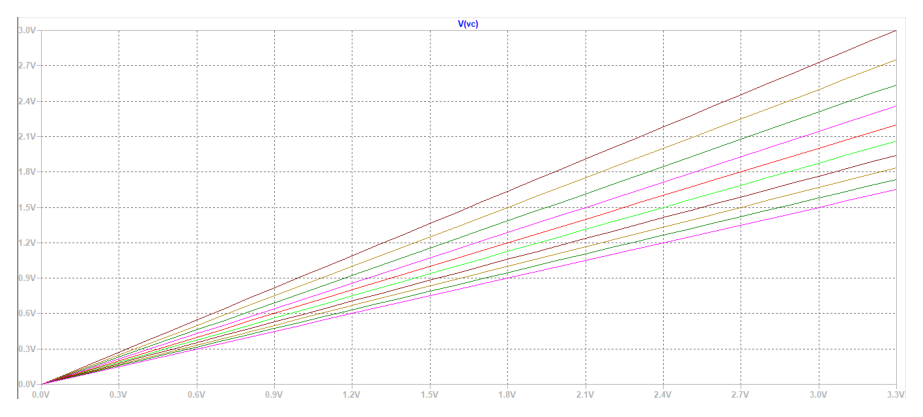
\includegraphics[width=1\textwidth]{graph_10k}
                \caption{Gráficas de voltaje de $R_{ref} = 10k\Omega$ con barrido en $R_{test}$}
                \label{fig:graph_10k}
            \end{figure}

\newpage
El diseño digital para la caracterización de resistencias se compone de varios módulos interconectados que permiten la adquisición y procesamiento de los datos.
Estos módulos son:


\begin{itemize}
    \item Memoria ROM: Contiene valores en binario correspondientes a voltajes de 0V a 3V, con incrementos de 0.1V. Este módulo está conectado al DAC para enviar los valores de voltaje al siguiente paso del sistema.

    \item Escritura del DAC: Convierte y transmite los voltajes generados por la ROM al circuito divisor de voltaje, permitiendo la caracterización de resistencias.

    \item Escritura y lectura del ADC: Lee y convierte el voltaje presente en $R_{ref}$. Los valores obtenidos son almacenados en la memoria RAM.

    \item Memoria RAM: Almacena los voltajes convertidos por el ADC. Su función principal es conservar el valor de la resistencia del microbolómetro en caso de cambios en la iluminación. La salida de la RAM se conecta a un multiplexor.

    \item Multiplexor: Organiza la salida de la RAM en grupos de 8 bits. Esto es necesario porque el multiplexor está conectado al módulo de transmisión RS232, que solo puede manejar datos en este formato.

    \item Transmisión (RS232): Envía los datos organizados por el multiplexor, almacenados en la RAM, hacia MATLAB para su posterior análisis.

    \item Contadores: Se utilizan dos contadores, uno para la memoria ROM y otro para la memoria RAM. Ambos son empleados para direccionar los datos de manera adecuada.

    \item Máquina de estados: Es el módulo más importante, compuesto por 17 estados, que se encarga de habilitar y coordinar el funcionamiento de todos los módulos anteriormente mencionados. A continuación, se explica la función de cada uno de los estados.
    \begin{enumerate}
     \item s0: La máquina de estados espera una señal de activación, la cual proviene de un push button.
     \item s1: Una vez activada, se habilita la escritura del DAC para iniciar el proceso de conversión de voltaje.
     \item s2: El DAC se deshabilita, y el sistema permanece en este estado mientras la bandera \textit{end of DAC} (eodac) sea cero. Cuando la bandera cambia a 1, indica que el DAC ha completado su conversión.
     \item s3 y s4: Estados de guarda que aseguran que el circuito divisor de voltaje esté correctamente polarizado.
     \item s5: Se activa el ADC para iniciar la lectura del voltaje de $R_{ref}$.
     \item s6: El ADC se desactiva, y el sistema permanece en este estado mientras la bandera \textit{end of ADC} (eodac) sea cero. Cuando cambia a 1, significa que el ADC ha terminado su conversión.
     \item s7: Se habilita la RAM y se almacena la conversión realizada por el ADC.
     \item s8: La RAM se deshabilita, y se incrementan los contadores de la ROM y la RAM.
     \item s9: El sistema mantiene el valor de los contadores y verifica si el contador de la RAM ha llegado a 31. Si es cierto, pasa al estado S10; si no, vuelve al estado S1.
     \item s10: Se reinician los contadores de la ROM y la RAM.
     \item s11: Se habilita el módulo de transmisión para comenzar a enviar datos.
     \item s12: La transmisión se deshabilita, y el sistema permanece en este estado hasta que la bandera \textit{end of transmission} (eotx) indique que se han enviado los 8 bits más significativos de la salida de la RAM. 
     \item s13: Se habilita nuevamente la transmisión, y el selector del multiplexor se pone a 1 para enviar los 8 bits menos significativos de la salida de la RAM.
     \item s14: La transmisión se desactiva, y el sistema espera hasta que se haya terminado de transmitir los bits restantes.
     \item s15: El contador de la RAM se incrementa para procesar el siguiente conjunto de datos.
     \item s16: El sistema mantiene el valor del contador de la RAM y verifica si ha llegado a 31. Si es cierto, se regresa al estado S0 para repetir el proceso; de lo contrario, se vuelve al estado S11 para continuar la transmisión.           
    \end{enumerate}
\end{itemize}


\subsection{Caracterización de matriz de resistencias}


\section{Caracterización de fotorresistencias}
\subsection{Caracterización de fotorresistencia}
En esta segunda etapa, se llevó a cabo la caracterización de una fotorresistencia, cuyo comportamiento es similar al de un microbolómetro. Esta similitud permitió utilizar la fotorresistencia como un medio de prueba para anticipar el funcionamiento del sistema con un microbolómetro real. El objetivo de esta fase fue observar y analizar cómo sería trabajar con un microbolómetro, permitiendo ajustar y validar los métodos utilizados en el sistema de adquisición de datos.


Para caracterizar la fotorresistencia, inicialmente se expuso a la iluminación de las lámparas de un salón. Sin embargo, debido a que el valor de la fotorresistencia no se estabilizaba, se optó por colocarla bajo condiciones "ideales". Para ello, la fotorresistencia se ubicó en una caja oscura, donde primero se midió su resistencia en ausencia de luz. Desafortunadamente, la resistencia aumentó tanto ($> 1M\Omega$) que el multímetro ya no pudo detectar su valor. Posteriormente, se decidió incorporar un LED de 3W, cuya intensidad se reguló utilizando un PWM. El LED se colocó en la parte superior de la caja, a 15cm de la fotorresistencia, permitiendo realizar mediciones bajo distintos condiciones controladas de luz.


El diseño digital para la caracterización de la fotorresistencia es similar al utilizado en la caracterización de resistencia, la única diferencia entre los diseños es la incorporación de un módulo PWM. El diseño de este módulo se basa en el uso de contadores y comparadores. Los contadores generan una señal periódica, mientras que los comparadores determinan el momento en el que la señal cambia de estado, ajustando así el tiempo en el que el LED permanece encendido durante cada ciclo.


El módulo PWM implementado cuenta con cuatro ciclos de trabajo: $25\%$, $50\%$, $75\%$ y $100\%$, lo que permite variar la intensidad del LED, además, de acuerdo con las especificaciones del LED, este se puede alimentar en un intervalo de voltaje de $3V - 3.8V$, por esta razón se optó por probar con tres voltajes de polarización distintos: $3V$, $3.3V$ y $3.5V$ y así determinar cual es el voltaje adecuado para polarizar al LED y qué ciclo de trabajo es mejor utilizar para una matriz de fotorresistencias. 


\subsection{Caracterización de matriz de fotorresistencias}
Al alimentar el LED con $3.3V$ y utilizando un ciclo de trabajo del $100\%$, se obtuvieron los valores de resistencia más apropiados, es por esto que, para la caracterización de una matriz de $2\times2$ fotorresistencias, el PWM mantuvo esta configuración, garantizando una iluminación constante sobre la matriz durante todo el proceso. En esta etapa, se emplearon los mismos bloques digitales que en la caracterización de la matriz de resistencias.

\section{Sistema de adquisición de datos}
Para la etapa final del sistema de adquisición de datos completo, se diseñó una PCB que alberga una matriz de 8x8 fototransistores, la cual es clave para la obtención de imágenes. En este proceso, muchos de los módulos utilizados en las etapas anteriores, como los convertidores y multiplexores, se emplean nuevamente para garantizar una lectura precisa de la matriz y la conversión de las señales en datos útiles para generar la imagen. En esta sección, se explicará tanto el diseño de la PCB como el diseño digital involucrado en la adquisición y procesamiento de las imágenes obtenidas mediante la matriz de fototransistores.

\subsection{Diseño de PCB}

\subsection{Diseño digital}


